\title{Robust non-stationary local slope estimation}
\renewcommand{\thefootnote}{\fnsymbol{footnote}}
\author{H. Wang, G. Huang, and Y. Chen
\thanks{Y. Chen, G. Huang, and Y. Chen are with Zhejiang University.}
\thanks{The research is supported by the starting fund from Zhejiang University.}}
\maketitle

\DeclareRobustCommand{\old}[1]{}
\DeclareRobustCommand{\new}[1]{#1}
\DeclareRobustCommand{\dlo}[1]{}
\DeclareRobustCommand{\wen}[1]{#1}

\begin{abstract}
The plane-wave destruction (PWD) method has been a widely used local slope estimation method in the seismic community. It is based on the discretization of the plane-wave partial differential equation (PWD) and the linearization of the PDE with respect to the local slope. Solving the linearized inverse problem for the slope perturbation is equivalent to solving a smoothness constrained optimization based on a shaping regularization method. The smoothness constraint in the shaping regularization is important in that it not only controls the stability and smoothness of the solution, i.e., slope perturbation, but also affects the accuracy and resolution of the solution. Traditional PWD algorithm is not easy to compromise the smoothness and resolution of the estimated local slope because it uses a stationary triangle smoothing operator as the shaping operator. Here, we propose to improve the robustness of the PWD algorithm by introducing a non-stationary triangle smoothing operator into the shaping regularization framework in order to adaptively constrain the solution according to the local signal reliability. The smoothing is weak in areas with a higher probability of signals and is strong in areas with a higher likelihood of noise. The smoothing radius can be adaptively estimated based on an optimization model, which is solved by a line-search method. The proposed new slope estimation method is referred to as a non-stationary method compared with the traditional stationary one. The effectiveness and benefits of the new slope estimation method are validated via several synthetic and field data examples.
\end{abstract}

\begin{keywords}
Seismic signal analysis, structural filtering, local slope
\end{keywords}

\section{Introduction}
The local slope is a seismic attribute that can be extracted from the raw data. It has been successfully applied in several geophysical processing and inverse problems, e.g., wavefield separation \cite{harlan1984signal,fomel2002pwd}, predictive painting \cite{fomel2010predictive}, velocity-independent seismic imaging \cite{fomel2007velocity}, regularized geophysical inversion \cite{fomel2007shape}, etc. 

\new{The local slope is closely related with the seismic dip angle. Researchers have started the seismic dip estimation from last century. There are at least three-generations methods for calculating the seismic dip \cite{chopra2007volumetric}, e.g., (1) cross-correlation based methods \cite{browaeys2010local,aqrawi2012hybrid,aarre2013consistent}, (2) semblance-based discrete scanning methods \cite{marfurt19983,lou2019accurate}, (3) structure tensor-based methods \cite{hale2007local,wu2017directional,wang2018robust}.}

In the past decades, there have been a variety of slope estimation methods \new{based on the plane-wave theory}. The plane-wave destruction (PWD) method was originally proposed by \cite{claerbout1992pvi}. Fomel (2002) \cite{fomel2002pwd} proposed to use an implicit finite difference scheme to discretize the plane-wave equation, where an infinite impulse response (IIR) filter (also known as the all-pass filter) to approximate the phase-shift operator and transforms the plane-wave equation into a non-linear inverse problem. Hale (2007) \cite{hale2007local} proposed the structure-tensor, also known as the gradient tensor \cite{van1995estimators}, \old{based slope estimation method based}\new{where the slope estimation is based} on the assumption that eigenvector corresponding to the largest eigenvalue of the structure tensor \old{point}\new{points} to the structural direction.  Liu et al. (2015) \cite{liuyang2015} took advantage of the relation between 2D Hilbert transform and the derivatives of the seismic data and derive a fast non-iterative dip estimation method, which turns to be more robust than the PWD based slope estimation method in the case of noisy data \cite{yangkang2018gji3}. Chen et al. (2013) \cite{zhonghuan2013accelerated} accelerated the PWD method by deriving an analytical solution to the non-linear inverse problem based on the three-point all-pass approximation filter, thus the PWD method no longer requires outer-loop non-linear iterations and thus is significantly accelerated. Chen et al. (2013) \cite{zhonghuan2013omnidirectional} further improved the conventional PWD algorithm by proposing a circle-interpolating model that makes the PWD method avoid the aliasing issues, thereby well handling both vertical and horizontal structures.

The local slope of a seismic data can be used to compress the seismic events along the slope direction, i.e., to obtain an optimally sparse representation of the seismic data. This sparsification process is referred to as the seislet transform \cite{fomel2010seislet}. Since the seislet transform is based on the structure direction to compress the data, its sparsity in the transform domain highly depends on the accuracy of the estimated local slope. Chen (2016) \cite{yangkang2016emd} discussed the influence of the error of local slope estimation in the sparsity performance of the seislet transform, and developed a dip-separated processing strategy to deal with the limitation of the PWD algorithm in the estimation of conflicting dips. 

One important application of slope is structural filtering. The basics of the structural filtering is to create a local window along the structural direction and then apply a mean/median filter within this local window. \new{Liu et al. (2010)} \cite{liuyang2010} proposed a trace-prediction way to create local windows along the structure direction by creating a third dimension with predicted traces following the slope. Gan et al. (2016) \cite{shuwei2016somf} developed a structure-oriented median filtering method to suppress the blending noise arise from the simultaneous-source acquisition, where the slope is estimated by transforming the NMO-picked velocities to the slope. Chen et al. (2019) \cite{sosvmf} developed a structure-oriented space-varying median filtering method to deal with the problem of unflattened events in the third  dimension when the slope of seismic data is not accurately estimated. 

Another important application of slope is to regularize the inversion-based seismic imaging approaches, e.g., the least-squares reverse time migration (LSRTM) and full waveform inversion (FWI). Xue et al. (2016) \cite{zhiguang2016} developed a constrained LSRTM method to deal with the intense migration artifacts caused by the simultaneous-source shooting or insufficient spatial data sampling, where the smoothing operator along the structural direction is used as a shaping operator to constrain the smoothness of the geological structures. Qu et al. (2019) \cite{qushan2019geo} developed a directional total variation (DTV) method to constrain the velocity model during the FWI iteration so as to avoid being trapped into a local minimum. The DTV constraint is equivalent to the rotated traditional total variation following the dip angle of the geological structure. 

Generally speaking, the PWD method has been a well-known slope estimation method in the exploration seismic community. However, the low anti-noise ability of the PWD method still limits its wide application in challenging situations where the random noise is strong \cite{curveletieee2016,yanan2014,weilin2017dlsp,shaohuan2018ieee,zhaoqiang2019tgrs,wang2019hankel}. From the parameter setting perspective, it is usually required to choose a large smoothing radius when dealing with a low signal-to-noise ratio so that the resulted local slope is sufficiently smooth, i.e., avoiding the unstable solution. However, a larger smoothing radius could degrade the fidelity of the estimated slope, resulting in a poor structural processing or constraint when applied subsequently for other tasks. Thus, the stationary fixed smoothing radius is rigid in tuning the performance of the PWD method. In this paper, we developed a novel non-stationary slope estimation method, where the triangle smoother used to regularize the smoothness of the slope is stretched and squeezed according to the signal reliability and complexity. For areas with higher signal reliability or a simpler structural complexity, we use a relatively smaller radius, and vice versa. More importantly, we introduce an adaptive smoothing radius estimation method based on an iterative optimization model. The non-stationary slope estimation with the adaptively estimated smoothing radius is tested via several synthetic and field datasets, which demonstrate a great potential of the proposed method in obtaining better performance in structurally filtering complex seismic data.  

\subsection{Plane-wave destruction (PWD)}
The PWD algorithm is based on the plane-wave approximation of the wave equation:
\begin{equation}
\label{eq:plane}
\sigma \frac{\partial d}{\partial t} + \frac{\partial d}{\partial x} = 0,
\end{equation}
where $d$ is the wavefield, $t$ and $x$ denotes time and space, respectively, and $\sigma$ denotes the local slope. 

A general solution to equation \ref{eq:plane} can be expressed as: 
\begin{equation}
\label{eq:plane}
d(t,x) = f(t-\sigma x),
\end{equation}
which indicates a two-point prediction filter in the frequency domain, i.e.,
\begin{equation}
\label{eq:plane1}
D(w,x) = e^{iw\sigma x}F(w),
\end{equation}
and
\begin{equation}
\label{eq:plane2}
D(w,x) = e^{iw\sigma }D(w,x-1) ,
\end{equation}
where $D(w,x)$ and $F(w)$ denote the spectrum of $d(t,x)$ and $f(t)$ in the frequency domain. It is clear that the two-point prediction filter to destruct equation \ref{eq:plane2} takes the form $[1,-e^{iw\sigma }]$. 

Equation \ref{eq:plane2} can be further transformed into the Z-transform notation as: 
\begin{equation}
\label{eq:Z}
A(Z_t,Z_x) D(Z_t,Z_x) = 0,
\end{equation}
where 
\begin{equation}
\label{eq:Z1}
A(Z_t,Z_x) = (1-Z_x\frac{L(Z_t)}{L(1/Z_t)}),
\end{equation}
or 
\begin{equation}
\label{eq:Z2}
H(Z_t,Z_x) D(Z_t,Z_x) = 0,
\end{equation}
where 
\new{\begin{equation}
\label{eq:Z3}
H(Z_t,Z_x) = (L(1/Z_t)-Z_xL(Z_t)),
\end{equation}}
$A(Z_t,Z_x)$ and $H(Z_t,Z_x)$ are two different forms of the plane-wave destruction filter in the Z-transform domain. $L(Z_t)/L(1/Z_t)$ is referred to as the Thiran all-pass filter \cite{thiran1971recursive,fomel2002pwd,zhonghuan2013accelerated}. 

\subsection{\old{Gaussian-Newton's}\new{Gauss-newton} method}
Thanks to the all-pass filter, the plane-wave equation is then transformed into a non-linear inverse problem. Thus, slope estimation is essentially to solve the non-linear inverse problem as expressed below:
\begin{equation}
\label{eq:nonlinear}
\mathbf{H}(\boldsymbol{\sigma})\mathbf{d}=\mathbf{0},
\end{equation}
where $\mathbf{H}(\boldsymbol{\sigma})$ denotes a convolutional operator and is a non-linear function with respect to the slope vector $\boldsymbol{\sigma}$. According to \old{Gaussian-Newton's}\new{Gauss-newton} method, equation \ref{eq:nonlinear} can be solved via
\begin{equation}
\label{eq:nonlinear2}
\boldsymbol{\sigma}_{n+1}=\boldsymbol{\sigma}_n-(\mathbf{J}^T\mathbf{J})^{-1}\mathbf{J}^T\mathbf{H}(\boldsymbol{\sigma}_n)\mathbf{d},
\end{equation}
where $\mathbf{J}$ is the Jacobian matrix with respect to variable vector $\boldsymbol{\sigma}$ corresponding to $\mathbf{H}(\boldsymbol{\sigma})\mathbf{d}$. Equation \ref{eq:nonlinear} indicates that during each non-linear iteration, there is an embedded iteration that aims to solve $(\mathbf{J}^T\mathbf{J})^{-1}$, which is the inversion of the \old{Hession matrix}\new{approximated Hessian matrix}. It is also equivalent to solving the following linear equation via a least-squares method:
\begin{equation}
\label{eq:nonlinear3}
\mathbf{H}(\boldsymbol{\sigma}_n)\mathbf{d} = \mathbf{J} \Delta \boldsymbol{\sigma}_n,
\end{equation}
where $\mathbf{J}$ can be expressed \old{\new{$\mathbf{J}=\mathbf{H}'(\boldsymbol{\sigma}_n)$}}\new{$\mathbf{J}=\mathbf{H}'(\boldsymbol{\sigma}_n)\mathbf{d}$}, $ \Delta \boldsymbol{\sigma}_n$ denotes the slope update during each non-linear iteration.  Here, $\mathbf{H}'$ denotes the derivative form of the PWD filter, e.g., each coefficient of $\mathbf{H}$ is taken a derivative.

\begin{figure}[htb!]
\centering
\subfigure[]{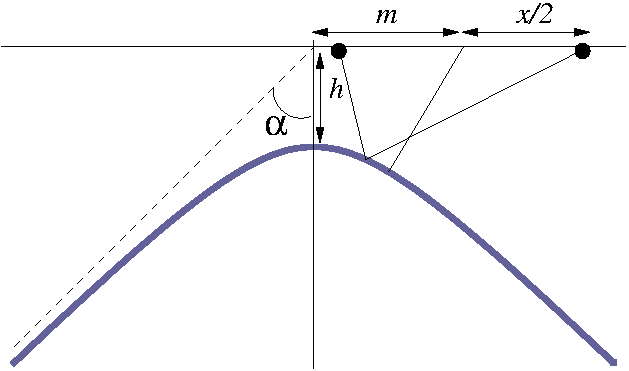
\includegraphics[width=0.45\columnwidth]{hyper/Fig/hyper}
   \label{fig:hyper}}
   \subfigure[]{\includegraphics[width=0.45\columnwidth]{hyper/Fig/hyper-n}
   \label{fig:hyper-n}}
\caption{Synthetic test. (a) Clean data. (b) Noisy data (SNR=1.56 dB). }
\label{fig:hyper,hyper-n}
\end{figure}

\begin{figure}[htb!]
\centering
\subfigure[]{\includegraphics[width=0.45\columnwidth]{hyper/Fig/hyper-dip}
  \label{fig:hyper-dip}}
  \subfigure[]{\includegraphics[width=0.45\columnwidth]{hyper/Fig/hypern-dip}
  \label{fig:hypern-dip}}\\
\subfigure[]{\includegraphics[width=0.45\columnwidth]{hyper/Fig/hypern-dip2}
  \label{fig:hypern-dip2}}
  \subfigure[]{\includegraphics[width=0.45\columnwidth]{hyper/Fig/hypern-dip3}
  \label{fig:hypern-dip3}}
\caption{Slope estimation results. (a) Estimated slope from the clean data with a constant smoothing radius $R=5$. (b) Estimated slope from the noisy data with a constant smoothing radius $R=8$. (c) Estimated slope from the noisy data with a constant smoothing radius $R=50$. (d) Estimated slope from the noisy data with the non-stationary smoothing radius map shown in Fig. \ref{fig:rectdip1}. Note that (b) and (c) use the smallest and largest smoothing radii of the non-stationary smoothing radius map. }
\label{fig:hyper-dip,hypern-dip,hypern-dip2,hypern-dip3}
\end{figure}

\begin{figure}[htb!]
 \centering
 \includegraphics[width=\columnwidth]{hyper/Fig/rectdip1}
  \caption{Adaptively estimated smoothing radius for non-stationary dip estimation.}
  \label{fig:rectdip1}
\end{figure}

\begin{figure}[htb!]
\centering
\subfigure[]{\includegraphics[width=0.45\columnwidth]{hyper/Fig/hypern-sm1}
   \label{fig:hypern-sm1}}
   \subfigure[]{\includegraphics[width=0.45\columnwidth]{hyper/Fig/hypern-sm2}
   \label{fig:hypern-sm2}}\\
\subfigure[]{\includegraphics[width=0.45\columnwidth]{hyper/Fig/hypern-sm3}
   \label{fig:hypern-sm3}}
   \subfigure[]{\includegraphics[width=0.45\columnwidth]{hyper/Fig/hypern-sm4}
   \label{fig:hypern-sm4}}\\
\caption{Smoothing test. (a) Structurally smoothed using the slope estimated from the clean data (SNR=13.73 dB). (b) Structurally smoothed using the slope estimated from the noisy data with a small constant smoothing radius (SNR=11.80 dB). (c) Structurally smoothed using the slope estimated from the noisy data with a large constant smoothing radius (SNR=10.71 dB). (d) Structurally smoothed using the slope estimated from the noisy data with non-stationary smoothing radius (SNR=13.11 dB).}
\label{fig:hypern-sm1,hypern-sm2,hypern-sm3,hypern-sm4}
\end{figure}

\begin{figure}[htb!]
\centering
\subfigure[]{\includegraphics[width=0.45\columnwidth]{hyper/Fig/hypern-sm1-n}
   \label{fig:hypern-sm1-n}}
   \subfigure[]{\includegraphics[width=0.45\columnwidth]{hyper/Fig/hypern-sm2-n}
   \label{fig:hypern-sm2-n}}\\
\subfigure[]{\includegraphics[width=0.45\columnwidth]{hyper/Fig/hypern-sm3-n}
   \label{fig:hypern-sm3-n}}
   \subfigure[]{\includegraphics[width=0.45\columnwidth]{hyper/Fig/hypern-sm4-n}
   \label{fig:hypern-sm4-n}}\\
\caption{Smoothing test. (a)-(d) Removed noise corresponding to Figs. \ref{fig:hypern-sm1}-\ref{fig:hypern-sm4}.}
\label{fig:hypern-sm1-n,hypern-sm2-n,hypern-sm3-n,hypern-sm4-n}
\end{figure}



\begin{figure}[htb!]
\centering
\subfigure[]{\includegraphics[width=0.45\textwidth]{real2d/Fig/g-0}
   \label{fig:g-0}}
   \subfigure[]{\includegraphics[width=0.45\textwidth]{real2d/Fig/g-z-a}
   \label{fig:g-z-a}}
\subfigure[]{\includegraphics[width=0.45\textwidth]{real2d/Fig/g-z-b}
   \label{fig:g-z-b}}
\caption{Field data example. (a) Raw field data. (b) Zoomed section A. (c) Zoomed section B.}
\label{fig:g-0,g-z-a,g-z-b}
\end{figure}

\begin{figure}[htb!]
\centering
\includegraphics[width=0.45\textwidth]{real2d/Fig/g-rectdip1}
\caption{Field data example. Non-stationary smoothing radius.}
\label{fig:g-rectdip1}
\end{figure}
   

\begin{figure}[htb!]
\centering
\subfigure[]{\includegraphics[width=0.45\textwidth]{real2d/Fig/g-dip1}
   \label{fig:g-dip1}}
   \subfigure[]{\includegraphics[width=0.45\textwidth]{real2d/Fig/g-dip2}
   \label{fig:g-dip2}}
\subfigure[]{\includegraphics[width=0.45\textwidth]{real2d/Fig/g-dip3}
   \label{fig:g-dip3}}
\caption{Smoothing test of the field data example. (a) Slope estimated from the noisy data with a small constant smoothing radius $R=8$. (b) Slope estimated from the noisy data with a large constant smoothing radius $R=100$. (c) Slope estimated from the noisy data with non-stationary smoothing radius.}
\label{fig:g-dip1,g-dip2,g-dip3}
\end{figure}


\begin{figure}[htb!]
\centering
\subfigure[]{\includegraphics[width=0.45\textwidth]{real2d/Fig/g-sm1-0}
  \label{fig:g-sm1-0}}
  \subfigure[]{\includegraphics[width=0.45\textwidth]{real2d/Fig/g-sm2-0}
  \label{fig:g-sm2-0}}
\subfigure[]{\includegraphics[width=0.45\textwidth]{real2d/Fig/g-sm3-0}
  \label{fig:g-sm3-0}}
\caption{Smoothing test of the field data example. (a) Structurally smoothed using the slope estimated from the noisy data with a small constant smoothing radius. (b) Structurally smoothed using the slope estimated from the noisy data with a large constant smoothing radius. (c) Structurally smoothed using the slope estimated from the noisy data with non-stationary smoothing radius.}
\label{fig:g-sm1-0,g-sm2-0,g-sm3-0}
\end{figure}

\begin{figure}[htb!]
\centering
\subfigure[]{\includegraphics[width=0.45\textwidth]{real2d/Fig/g-sm1-n}
  \label{fig:g-sm1-n}}
  \subfigure[]{\includegraphics[width=0.45\textwidth]{real2d/Fig/g-sm2-n}
  \label{fig:g-sm2-n}}
\subfigure[]{\includegraphics[width=0.45\textwidth]{real2d/Fig/g-sm3-n}
  \label{fig:g-sm3-n}}
\caption{Smoothing test of the field data example. (a)-(c) Removed noise corresponding to Figs. \ref{fig:g-sm1-0}-\ref{fig:g-sm3-0}.}
\label{fig:g-sm1-n,g-sm2-n,g-sm3-n}
\end{figure}

\begin{figure}[htb!]
\centering
\subfigure[]{\includegraphics[width=0.45\textwidth]{real2d/Fig/g-sm1-z-a0}
 \label{fig:g-sm1-z-a0}}
 \subfigure[]{\includegraphics[width=0.45\textwidth]{real2d/Fig/g-sm2-z-a0}
 \label{fig:g-sm2-z-a0}}
\subfigure[]{\includegraphics[width=0.45\textwidth]{real2d/Fig/g-sm3-z-a0}
 \label{fig:g-sm3-z-a0}}
\caption{Zoomed comparison of the field data example (frame box A). (a) Structurally smoothed using the slope estimated from the noisy data with a small constant smoothing radius. (b) Structurally smoothed using the slope estimated from the noisy data with a large constant smoothing radius. (c) Structurally smoothed using the slope estimated from the noisy data with non-stationary smoothing radius.}
\label{fig:g-sm1-z-a0,g-sm2-z-a0,g-sm3-z-a0}
\end{figure}

\begin{figure}[htb!]
\centering
\subfigure[]{\includegraphics[width=0.45\textwidth]{real2d/Fig/g-sm1-z-b0}
  \label{fig:g-sm1-z-b0}}
  \subfigure[]{\includegraphics[width=0.45\textwidth]{real2d/Fig/g-sm2-z-b0}
  \label{fig:g-sm2-z-b0}}
\subfigure[]{\includegraphics[width=0.45\textwidth]{real2d/Fig/g-sm3-z-b0}
  \label{fig:g-sm3-z-b0}}
\caption{Zoomed comparison of the field data example (frame box B). (a) Structurally smoothed using the slope estimated from the noisy data with a small constant smoothing radius. (b) Structurally smoothed using the slope estimated from the noisy data with a large constant smoothing radius. (c) Structurally smoothed using the slope estimated from the noisy data with non-stationary smoothing radius.}
\label{fig:g-sm1-z-b0,g-sm2-z-b0,g-sm3-z-b0}
\end{figure}

\subsection{Shaping regularization with non-stationary smoothing}
To ensure the smoothness and stability of the slope update, we use the following shaping regularization to solve the linear inverse problem expressed in equation \ref{eq:nonlinear3}:
\begin{equation}
\label{eq:linear}
\Delta \boldsymbol{\sigma}_n^{m} = \mathbf{S}\left[ \Delta \boldsymbol{\sigma}_n^{m-1} + \mathbf{J}^T\left( \mathbf{H}(\boldsymbol{\sigma}_n)\mathbf{d} - \mathbf{J}\Delta \boldsymbol{\sigma}_n^{m-1}\right)\right],
\end{equation}
where $\Delta \boldsymbol{\sigma}_n^{m}$ denotes the estimated $\Delta \boldsymbol{\sigma}_n$ after $m$th linear iteration. $\mathbf{S}$ is a shaping operator used to constrain the model behavior and ensure a fast convergence. The converged model based on the shaping regularization method is given as:
\begin{equation}
\label{eq:shape}
\hat{\Delta \boldsymbol{\sigma}_n} = \mathbf{T}[\lambda^2\mathbf{I} + \mathbf{T}^T(\mathbf{J}^T\mathbf{J}-\lambda^2\mathbf{I})\mathbf{T}]^{-1}\mathbf{T}^T\mathbf{J}^T\mathbf{H}(\boldsymbol{\sigma}_n)\mathbf{d},
\end{equation}
where $\mathbf{T}$ denotes a triangle smoothing operator. \new{In equation \ref{eq:linear}, the shaping operator is chosen as $\mathbf{S}=\mathbf{T}\mathbf{T}^T$. $\lambda$ is a scaling parameter that controls the relative scaling of the forward operator $\mathbf{J}$ \cite{fomel2007shape}. } The triangle smoothing operator takes the following form in the Z transform domain:
\begin{equation}
\label{eq:T}
T(Z) = B(Z)B(Z),
\end{equation} 
where $T(Z)$ and $B(Z)$ denote the triangle and rectangle smoothers in the Z-transform notations, respectively. The rectangle smoother can be expressed in the following way:
\begin{equation}
\label{eq:BZ}
B(Z)=\frac{1-Z^N}{1-Z} = 1 + Z + Z^2 +\cdots + Z^{N-1}.
\end{equation} 
Implementation of the rectangle smoothing \ref{eq:BZ} can be efficient when using a recursive strategy. For example, division by $1-Z$ corresponds to a causal integration operation in the time domain; multiplying \new{by} $1-Z^N$ in the numerator of equation \ref{eq:BZ} is equivalent to implementing the following recursion:
\begin{equation}
\label{eq:recur}
y_n = x_1 - x_{N},
\end{equation}
where $N$ denotes the smoothing radius. Thus, given a non-stationary distribution map of the smoothing radius, we can obtain a very fast implementation of the non-stationary smoothing following equations \ref{eq:T}-\ref{eq:recur}. 

The non-stationary smoothing radius can either be defined with help of a priori information, or be calculated by utilizing the concept of signal reliability, e.g., introduced in \cite{liuyang2009tvmf} and \cite{sosvmf}. The signal reliability simply means the possibility of a point as a signal point. In the signal point, it is helpful to use a smaller smoothing radius for better signal preservation, and for a noise point, it is better to use a long smoothing radius for an exclusive removal of the noise.  Here, we introduce a new method for adaptively estimating the non-stationary smoothing radius based on optimization. 

We can formulate the following optimization method in order to estimate the adaptive smoothing radius:
\new{\begin{equation}
\label{eq:nsm}
O= \parallel \mathcal{L}\left(\mathbf{T}(\mathbf{n})\mathbf{d}\right) - \mathcal{L}(\mathbf{d}_B) \parallel_2^2, 
\end{equation}}
where $O$ denotes the objective function of the optimization problem \cite{greer2018matching}. $\mathcal{L}$ denotes a local attribute estimator, e.g., the local frequency attribute \cite{fomel2007localattr}, $\mathbf{T}(\mathbf{n})$ denotes the triangle smoothing operator that is a function of the non-stationary smoothing radius vector $\mathbf{n}$, $\mathbf{d}$ denotes the input data, and $\mathbf{d}_B$ denotes a lowpass filter\new{, where the cut-off frequency could be chosen as the dominant frequency of the seismic data}. %The idea is similar to that was proposed in , where the low-frequency legacy seismic data is merged to the high-resolution data with a non-stationary smoothing. 
\new{The local attribute estimator is chosen as the local frequency operator, which is a local version of the instantaneous frequency operator. It transforms the direct division of the instantaneous frequency operator as a regularized inverse problem, which is then solved via the shaping regularization method. The smoothing operator $\mathbf{T}$ is expressed in equation \ref{eq:T} as a Z-transform form.  }


We use a simple line-search method for minimizing the objective function expressed in equation \ref{eq:nsm}:
\begin{equation}
\label{eq:nsm2}
\mathbf{n}_{m} = \mathbf{n}_{m-1} + \alpha_m \left( \mathcal{S}\left(\mathbf{T}(\mathbf{n})\mathbf{d}\right) - \mathcal{S}(\mathbf{d}_B) \right),
\end{equation}
where $\alpha_m$ denotes a step size, gradually decreasing a larger value, e.g., 0.8, to a smaller value, e.g., 0.05, for a fast convergence. 

Note that the adaptive smoothing radius estimation method introduced here is an option to obtain a rough estimate of the optimal smoothing radius from a raw seismic data. In later examples, we will demonstrate the effectiveness of the optimization in estimating plausible smoothing radius distribution. However, an in-depth analysis of the optimization in terms of the theoretical implications, stability, and convergence is beyond the scope of this paper. Other options on obtaining non-stationary smoothing radius are worth investigating. To summarize, incorporating this adaptive smoothing radius estimation method into the recursion-based fast non-stationary smoothing can help better constrain the slope estimation by better compromising the smoothness of the result and the fidelity of the estimated slope. 

\section{Examples}
We use several synthetic and field data examples to demonstrate how the new slope estimation with non-stationary smoothing radius help improve the accuracy of the slope estimation, especially in the case of strong random noise. 

The first example is a synthetic test. The synthetic data is shown in Fig. \ref{fig:hyper,hyper-n} with the clean data on the left and the noisy data on the right. The signal-to-noise ratio (SNR) of the noisy data is 1.56 dB, based on the definition expressed below \cite{benfeng2019efficient}:
\begin{equation}
\label{eq:diff}
\text{SNR}=10\log_{10}\frac{\Arrowvert \mathbf{d} \Arrowvert_2^2}{\Arrowvert \mathbf{d} -\mathbf{d}_t\Arrowvert_2^2},
\end{equation}
where $\mathbf{d}$ denotes the ground-truth solution, i.e., the clean data in Fig. \ref{fig:hyper}, \new{and} $\mathbf{d}_t$ denotes the target signal to be evaluated. 

A comparison of different slope estimation results is shown in Fig. \ref{fig:hyper-dip,hypern-dip,hypern-dip2,hypern-dip3}. Fig. \ref{fig:hyper-dip} shows the estimated slope from the clean data with a constant smoothing radius $R=5$, which is considered as the ground-truth solution for the slope. Here, we use the traditional PWD algorithm \cite{fomel2002pwd} for the slope estimation. \new{To numerically compare the accuracy of slope, we treat the slope calculated from the clean data as the ground truth, and also use the SNR metric (defined in equation \ref{eq:diff}) for the evaluation.} Fig. \ref{fig:hypern-dip} shows the estimated slope from the noisy data with a constant smoothing radius $R=8$. It is clear that when using a smoothing radius $R=8$, the estimated local slope is highly unstable. There are a lot of artifacts in the slope map caused by the strong random noise. Note that a smaller smoothing radius will result in an even more unstable slope estimation result. \new{The accuracy of this slope result is 0.48 dB. } Fig. \ref{fig:hypern-dip2} shows the slope estimation result using a much larger smoothing radius $R=50$. \new{The accuracy of this slope result is 8.40 dB. } The resultant slope becomes stable and smooth across the whole profile, but the accuracy of the slope value in each point is significantly decreased. In addition, because of the larger smoothing radius, the PWD algorithm loses the resolution in distinguishing between seismic events. From the two results plotted in Figs. \ref{fig:hypern-dip} and \ref{fig:hypern-dip2}, we conclude that the resolution is maintained when the smoothing radius is small and is deteriorated when the radius becomes large. However, when the smoothing radius is small, the slope estimation is more unstable. Thus, the smoothing radius affects greatly the resolution and the stability of the estimated slope. It is always a compromise to achieve a balance between the smoothness and resolution of the slope map. Fig. \ref{fig:hypern-dip3} shows the estimated slope using the proposed method, which obtains a good compromise between the smoothness and the resolution of the slope map. \new{The accuracy of proposed slope result is 10.44 dB. } It is clear that the estimated slope using the proposed method is very close to the ground-truth solution of the slope estimation. 
 
Based on the aforementioned adaptive radius estimation method, we calculate the non-stationary radius map and show it in Fig. \ref{fig:rectdip1}. The minimum radius in this non-stationary radius map is about 8 and the maximum radius is about 50. Comparing the non-stationary radius map and the seismic data (Fig. \ref{fig:hyper}), we find that the adaptive smoothing radius estimation method correctly finds the areas of the signal components and output smaller radius for these signal areas and output a larger radius for other areas. It is clear that the proposed method adjusts the smoothing radius between the largest one (e.g., 50) and the smallest one (e.g., 8) in an adaptive way, and thus obtain a good compromise between the resolution (signal areas) and smoothness (noise areas) when estimating the local slope based on the PWD algorithm. Then, to compare the accuracy of the estimated local slope maps, we conduct a structure-oriented smoothing test. In the structure-oriented smoothing method \cite{sosvmf}, we first flat the seismic data based on a trace prediction strategy, and then apply a common triangle smoothing operator to the flattened dimension. 
The smoothed data using the four slope maps (Fig. \ref{fig:hyper-dip,hypern-dip,hypern-dip2,hypern-dip3}) are plotted in Fig. \ref{fig:hypern-sm1,hypern-sm2,hypern-sm3,hypern-sm4}. Fig. \ref{fig:hypern-sm1} plots the smoothed data using the ground-truth slope (Fig. \ref{fig:hyper-dip}). Fig. \ref{fig:hypern-sm2} corresponds to the local slope using a constant smoothing radius $R=8$ (Fig. \ref{fig:hypern-dip}). Because of the highly unstable artifacts in the local slope shown in Fig. \ref{fig:hypern-dip}, there are also some artifacts in the smoothed data, e.g., around 1.5s at the 100th trace.  Fig. \ref{fig:hypern-sm3} shows the smoothed data using the local slope with a constant smoothing radius $R=50$. It is clear that because of the low accuracy of the slope value caused by an over-large smoothing radius, the smoothing damages the signal amplitude significantly, e.g., the first seismic event. Fig.  \ref{fig:hypern-sm4} plots the smoothed data using the local slope estimated based on the proposed method. The result is very close to the smoothing result based on the ground-truth slope (Fig. \ref{fig:hypern-sm1}), and there are no observable artifacts and signal damages. Thus, we deem the smoothing result based on the proposed method accurate. The calculated SNRs for Figs. \ref{fig:hypern-sm1}-\ref{fig:hypern-sm4} are 13.73 dB, 11.80 dB, 10.71 dB, and 13.11 dB, respectively. It indicates \new{that} the smoothed data based on the proposed method obtains the highest SNR.  The removed noise sections caused by different smoothing operations are plotted in Fig. \ref{fig:hypern-sm1-n,hypern-sm2-n,hypern-sm3-n,hypern-sm4-n}. All the noise sections except for Fig. \ref{fig:hypern-sm3-n} shows no observable signal energy. However, there is \new{a} clear spatially coherent energy in Fig. \ref{fig:hypern-sm3-n}, which indicates a strong damage to the useful signals caused by the over-smoothed slope estimation when using a large constant smoothing radius $R=50$.

The second example is a \new{2D} field data test. The field data is shown in Fig. \ref{fig:g-0}. This field data has 2501 time samples and \old{2000}\new{1000} traces. The sampling rate is 2ms. Figs. \ref{fig:g-z-a} and \ref{fig:g-z-b} are two zoomed sections from the raw data for a detailed comparison. The two zooming areas are pointed by the two pink rectangles A and B. We show the adaptively estimated smoothing radius map in Fig. \ref{fig:g-rectdip1}. The non-stationary smoothing radius map successfully classifies the whole seismic section into signal areas where the smoothing radius is large and noise areas where the smoothing radius is small. The smallest smoothing radius on the map is about 8 and the largest smoothing radius is about 100. We apply different slope estimation methods to the noisy field data and get the slope maps in Fig. \ref{fig:g-dip1,g-dip2,g-dip3}. Fig. \ref{fig:g-dip1} shows the estimated slope using a small constant smoothing radius $R=8$, which is highly non-stable. Fig. \ref{fig:g-dip2} shows the estimated slope using a large constant smoothing radius $R=100$, which is somewhat over-smoothing. Fig. \ref{fig:g-dip3} shows the slope estimation result using the proposed method with the non-stationary smoothing radius presented in Fig. \ref{fig:g-rectdip1}. It is obvious the estimated slope using the proposed method is both smooth and \old{high-resolution}\new{with a high resolution}, maintaining the most subtle structures in the whole section. We then apply the structure-oriented smoothing based on different slope maps shown in Fig. \ref{fig:g-dip1,g-dip2,g-dip3}. The three smoothed profiles are plotted in Fig. \ref{fig:g-sm1-0,g-sm2-0,g-sm3-0}, with the top two results corresponding to the stationary slope estimation with a small smoothing radius \old{(left)}\new{(up)} and a large smoothing radius \old{(right)}\new{(down)}. The bottom \old{Fig.}\new{figure} corresponds to the result of the proposed method. The removed noise sections corresponding to the smoothed data are plotted in Fig. \ref{fig:g-sm1-n,g-sm2-n,g-sm3-n} for better evaluation. For a clearer comparison, we zoom in two sections from each \old{subFig.}\new{subfigure} in Fig. \ref{fig:g-sm1-0,g-sm2-0,g-sm3-0}. Fig. \ref{fig:g-sm1-z-a0,g-sm2-z-a0,g-sm3-z-a0} shows a comparison of the zoomed frame box A. From Fig. \ref{fig:g-sm1-z-a0,g-sm2-z-a0,g-sm3-z-a0}, it is clear that the top two results are both over-smoothed, causing either smoothing artifacts across the section \old{(left)}\new{(up)}, or damaged energy in areas with large dips \old{(right)}\new{(down)}. For example, several arrows point out the obvious distortion and damages to the useful seismic events in the top two panels. The smoothed data in the bottom panel seems to well preserve the key structures.  Fig. \ref{fig:g-sm1-z-b0,g-sm2-z-b0,g-sm3-z-b0} shows a comparison of the zoomed frame box B.  In this comparison, it is much more obvious that the top two results are over-smoothed seriously, as indicated by the white arrows. The result from the proposed method, however, still maintains the main geological structures. 

\new{The third example is a 3D field data test. The 3D field data is shown in Fig. \ref{fig:real}. The size of this dataset is $512\times 128\times 32$. This field data contains strong random noise. The adaptively calculated non-stationary smoothing radius is plotted in Fig. \ref{fig:rect1}. We apply different slope estimation methods to the noisy field data and get the slope maps in Fig. \ref{fig:real-s2dip1,real-s1dip1,real-ndip1}. The top two results correspond to the traditional PWD algorithm with constant smoothing radii. Fig. \ref{fig:real-s2dip1} shows the estimated slope using a small constant smoothing radius $R=2$, which is highly non-stable. Fig. \ref{fig:real-s1dip1} shows the estimated slope using a large constant smoothing radius $R=20$, which is over-smoothed. Fig. \ref{fig:real-ndip1} shows the slope estimation result using the proposed method with the non-stationary smoothing radius presented in Fig. \ref{fig:rect1}. It is obvious the estimated slope using the proposed method is both smooth and high-resolution, maintaining the most subtle structures in the whole section. We then apply the structure-oriented smoothing based on different slope maps. The three smoothed profiles are plotted in Fig. \ref{fig:real-pws2-0,real-pws1-0,real-pws3-0}, with the top two results corresponding to the stationary slope estimation with a small smoothing radius (up) and a large smoothing radius (down). The bottom figure corresponds to the result of the proposed method. The removed noise sections corresponding to the smoothed data are plotted in Fig. \ref{fig:real-pws2-n-0,real-pws1-n-0,real-pws3-n-0} for better evaluation.  As highlighted by the arrows in Fig. \ref{fig:real-pws2-0,real-pws1-0,real-pws3-0}. The proposed slope estimation method helps obtain the best denoising result. As highlighted by the arrows in Fig. \ref{fig:real-pws2-n-0,real-pws1-n-0,real-pws3-n-0}, a large smoothing radius would cause a over-smoothing in the denoised result and a small smoothing radius would cause an insufficient amount of removed noise. The proposed method, however, obtains the best compromise between noise removal and signal preservation.}

\section{Conclusion}
The traditional PWD method is based on a stationary smoothing shaping operator. The stationary smoothing shaping operator constrains the slope perturbation during each non-linear iteration. The constant smoothing radius is not convenient to choose in order to compromise the smoothness of the estimated slope field and its resolution. The unsatisfactory choice of the constant smoothing radius will result in unacceptable slope estimation results, which further deteriorate the structural filtering based on the accuracy of the local slope. The non-stationary smoothing based slope estimation method can overcome the limitation in choosing the fixed smoothing radius because the smoothing radius can be adaptively calculated based on an optimization method. We have shown that the smoothing radius plays an important role in the accuracy of the estimated slope and the proposed non-stationary slope estimation method can obtain a fairly accurate slope field in an adaptive way. Both synthetic and field data examples show the proposed non-stationary method can work effectively well in the case of strong random noise. The structure-oriented smoothing based upon the estimated local slope maps further verifies the advantages of the non-stationary smoothness constrained iterative slope estimation over the traditional PWD method. 


\begin{figure}[htb!]
\centering
\includegraphics[width=0.45\textwidth]{real3d/Fig/real}
\caption{\new{3D field data example.} }
\label{fig:real}
\end{figure}

\begin{figure}[htb!]
\centering
\includegraphics[width=0.45\textwidth]{real3d/Fig/rect1}
\caption{\new{3D field data example. Non-stationary smoothing radius.}}
\label{fig:rect1}
\end{figure}
   

\begin{figure}[htb!]
\centering
\subfigure[]{\includegraphics[width=0.45\textwidth]{real3d/Fig/real-s2dip1}
   \label{fig:real-s2dip1}}
   \subfigure[]{\includegraphics[width=0.45\textwidth]{real3d/Fig/real-s1dip1}
   \label{fig:real-s1dip1}}
\subfigure[]{\includegraphics[width=0.45\textwidth]{real3d/Fig/real-ndip1}
   \label{fig:real-ndip1}}
\caption{\new{Slope comparison of the 3D field data example. (a) Slope estimated from the noisy data with a small constant smoothing radius $R=2$. (b) Slope estimated from the noisy data with a large constant smoothing radius $R=20$. (c) Slope estimated from the noisy data with non-stationary smoothing radius.}}
\label{fig:real-s2dip1,real-s1dip1,real-ndip1}
\end{figure}


\begin{figure}[htb!]
\centering
\subfigure[]{\includegraphics[width=0.45\textwidth]{real3d/Fig/real-pws2-0}
  \label{fig:real-pws2-0}}
  \subfigure[]{\includegraphics[width=0.45\textwidth]{real3d/Fig/real-pws2-0}
  \label{fig:real-pws2-0}}
\subfigure[]{\includegraphics[width=0.45\textwidth]{real3d/Fig/real-pws3-0}
  \label{fig:real-pws3-0}}
\caption{\new{Smoothing test of the field data example. (a) Structurally smoothed using the slope estimated from the noisy data with a small constant smoothing radius. (b) Structurally smoothed using the slope estimated from the noisy data with a large constant smoothing radius. (c) Structurally smoothed using the slope estimated from the noisy data with non-stationary smoothing radius. Note the difference highlighted by the arrows.}}
\label{fig:real-pws2-0,real-pws1-0,real-pws3-0}
\end{figure}

\begin{figure}[htb!]
\centering
\subfigure[]{\includegraphics[width=0.45\textwidth]{real3d/Fig/real-pws2-n-0}
  \label{fig:real-pws2-n-0}}
  \subfigure[]{\includegraphics[width=0.45\textwidth]{real3d/Fig/real-pws1-n-0}
  \label{fig:real-pws1-n-0}}
\subfigure[]{\includegraphics[width=0.45\textwidth]{real3d/Fig/real-pws3-n-0}
  \label{fig:real-pws3-n-0}}
\caption{\new{Smoothing test of the field data example. (a)-(c) Removed noise corresponding to Figs. \ref{fig:real-pws2-0}-\ref{fig:real-pws3-0}. Note the difference highlighted by the arrows.}}
\label{fig:real-pws2-n-0,real-pws1-n-0,real-pws3-n-0}
\end{figure}


\section{Acknowledgments} 
We would like to thank S. Zu, D. Zhang, and S. Fomel for inspiring discussions. \new{We also thank two anonymous reviewers for constructive suggestions.}


\bibliographystyle{IEEEtran}
\bibliography{dip}



%\begin{figure}[htb!]
%	\centering
%	\subfigure[]{\includegraphics[width=0.8\textwidth]{Fig/fig}}
%	\caption{Caption.}
%	\label{fig:fig}
%\end{figure}


%\begin{figure}[htb!]
%	\centering
%	\subfigure[]{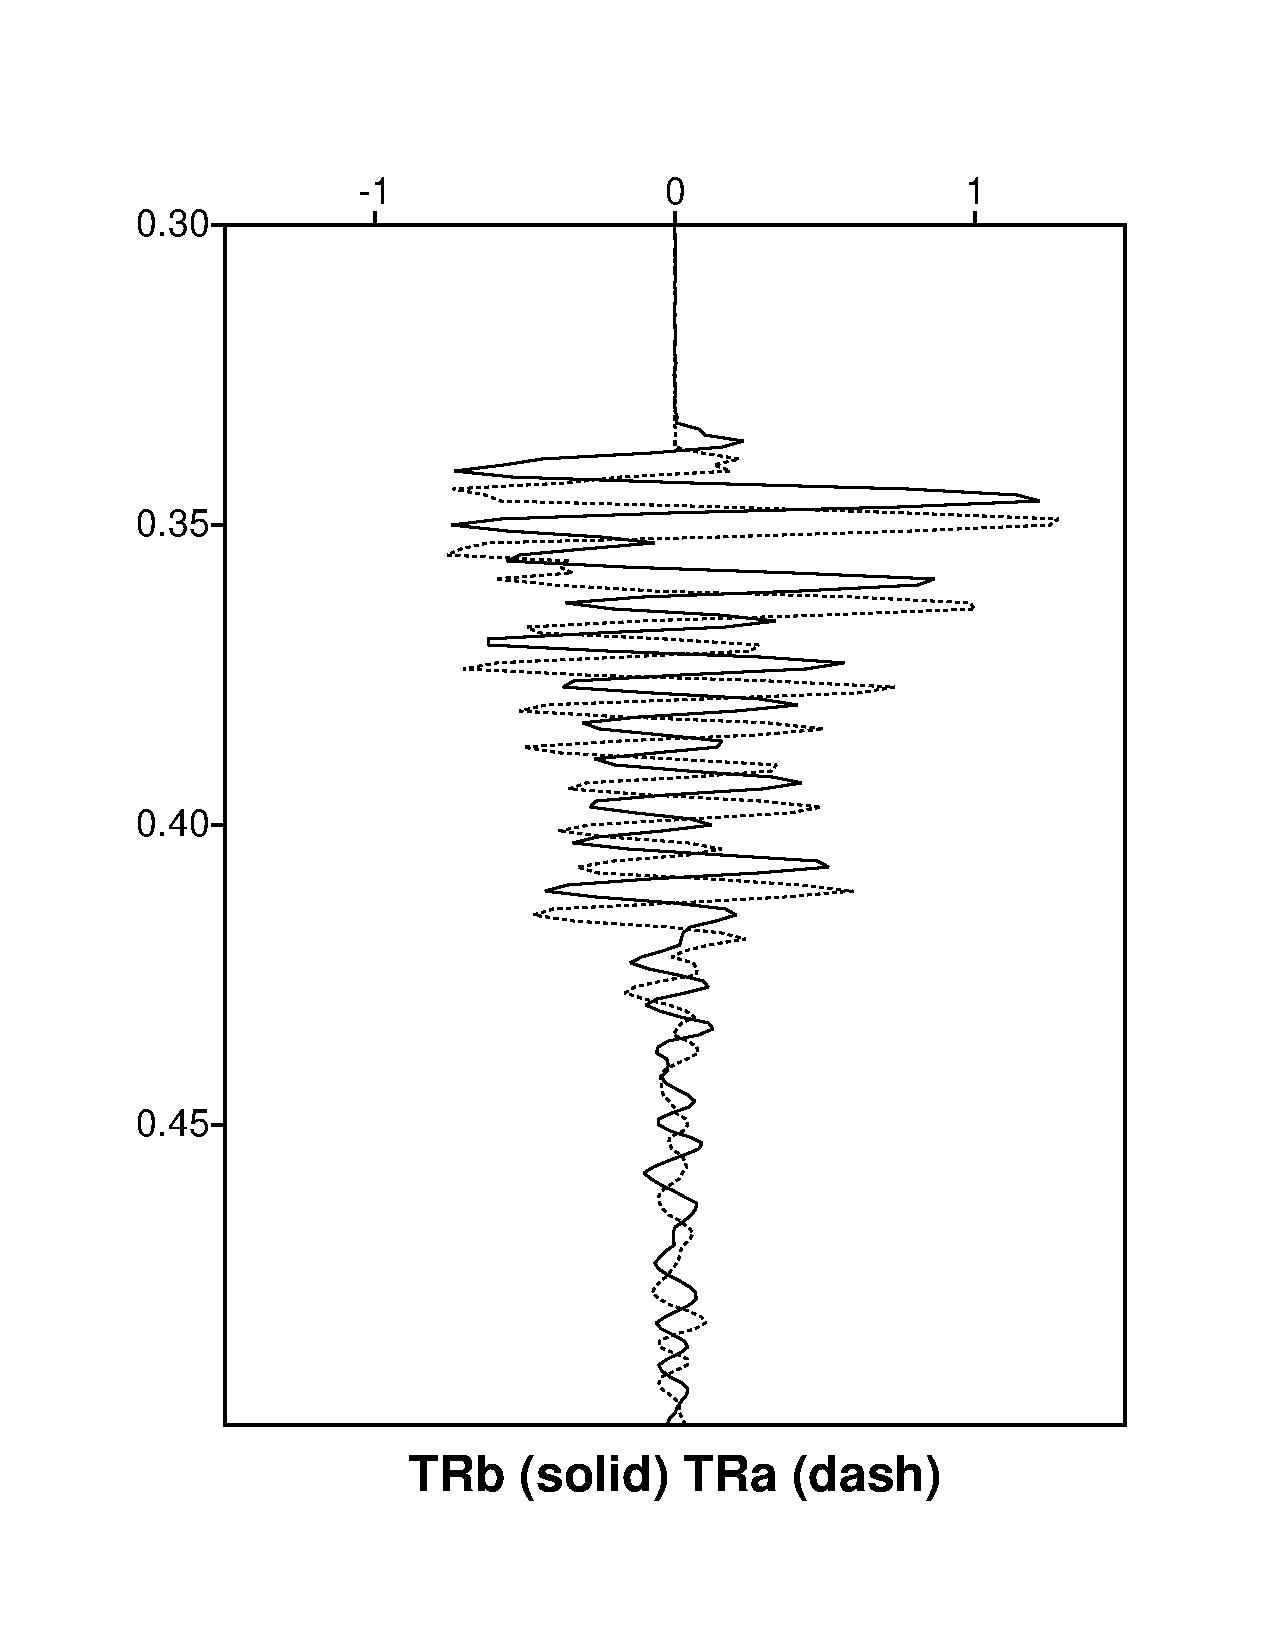
\includegraphics[width=0.45\textwidth]{Fig/fig1}}\\
%    \subfigure[]{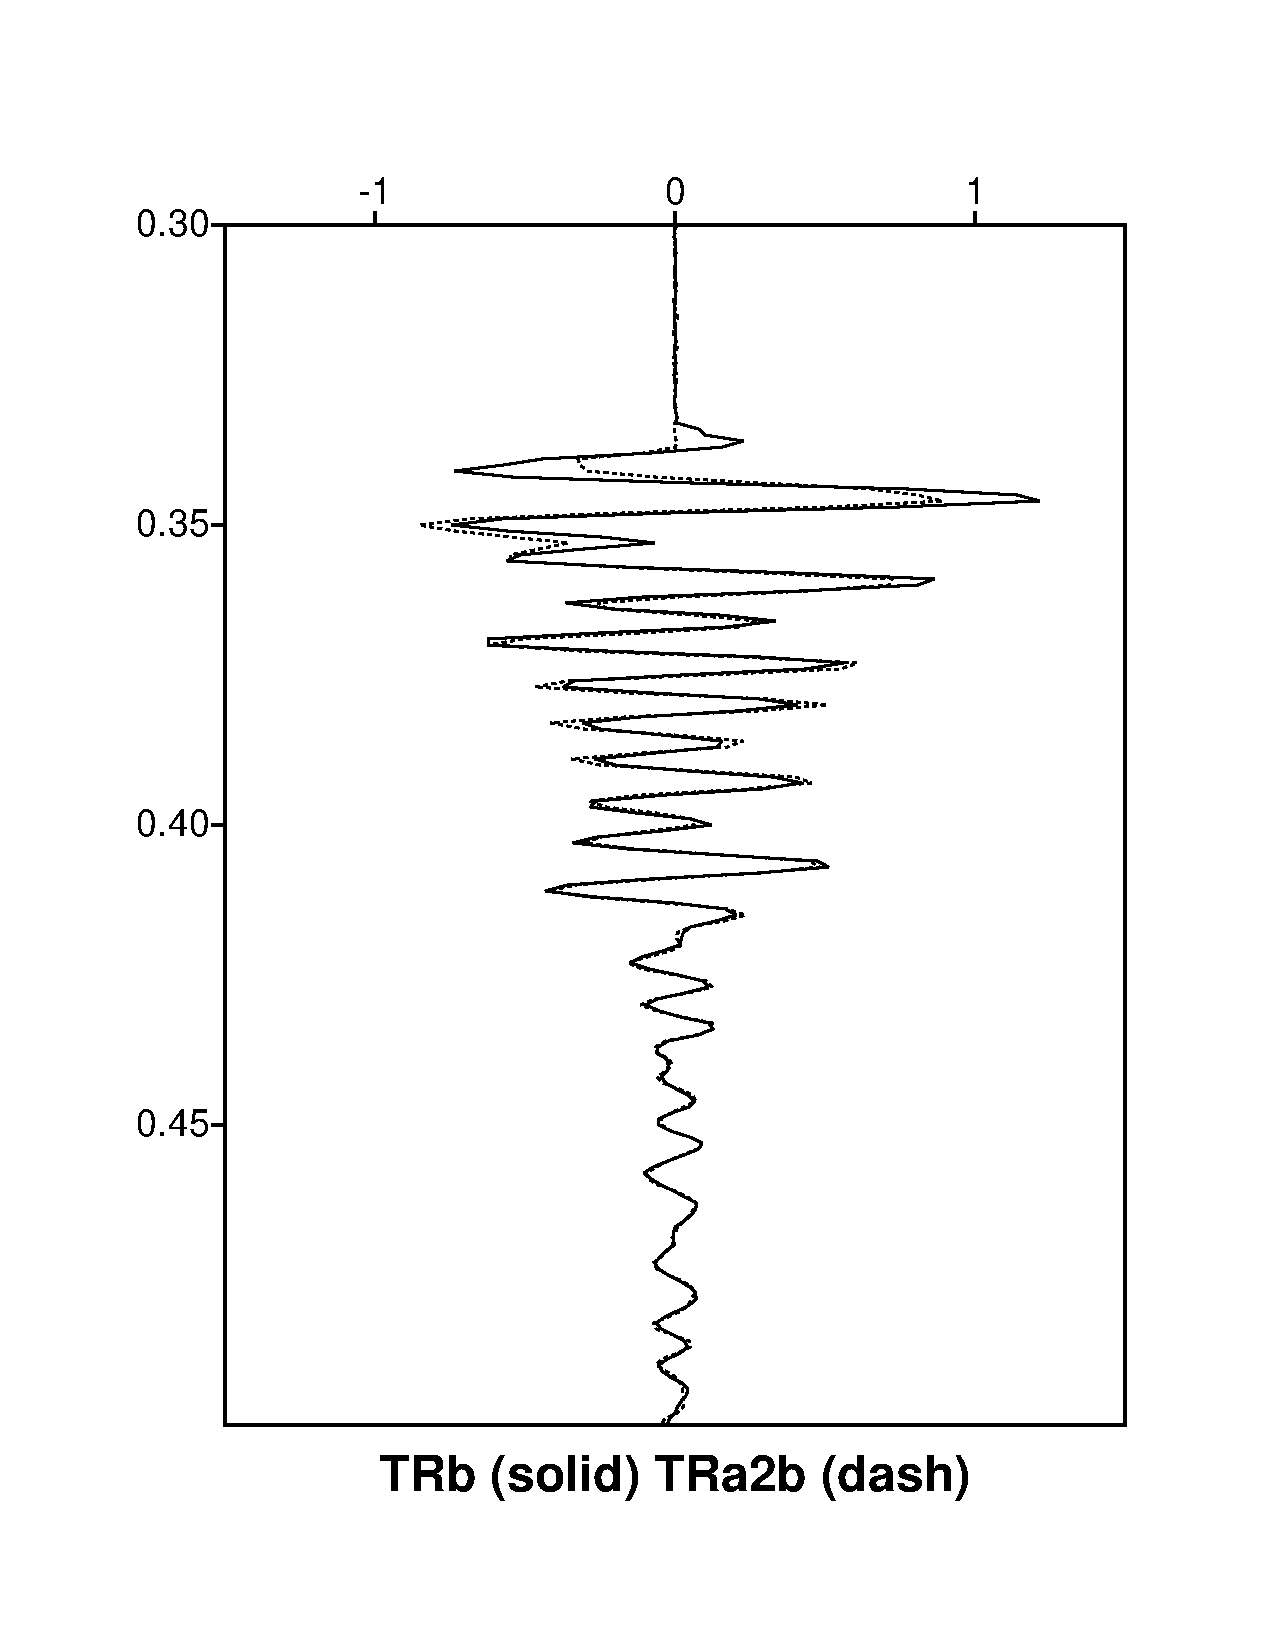
\includegraphics[width=0.45\textwidth]{Fig/fig2}}
%	\caption{(a) Caption a. (b) Caption b.}
%	\label{fig:fig1,fig2}
%\end{figure}

%\begin{table}[h]
%\caption{Table caption}
%\begin{center}
%     \begin{tabular}{|c|c|c|c|c|c|} 
%	  \hline Column1 (unit)  & Column2 (unit) & Column3 (unit) \\ 
%	  \hline 1 & 2  & 3 \\
%       \hline
%    \end{tabular} 
%\end{center}
%\label{tbl:table1}
%\end{table}





